
%%%%%%%%%%%%%%%%%%%%%%%%%%%%%%%%%%%%%%%%%%%%%%%%%%%%%%%%
%
% Copyright (c) 2003-2010 by University of Queensland
% Earth Systems Science Computational Center (ESSCC)
% http://www.uq.edu.au/esscc
%
% Primary Business: Queensland, Australia
% Licensed under the Open Software License version 3.0
% http://www.opensource.org/licenses/osl-3.0.php
%
%%%%%%%%%%%%%%%%%%%%%%%%%%%%%%%%%%%%%%%%%%%%%%%%%%%%%%%%

\section{Seismic Wave Propagation in Two Dimensions}

\sslist{example08a.py}
We will now expand upon the previous chapter by introducing a vector form of
the wave equation. This means that the waves will have not only a scalar
magnitude as for the pressure wave solution, but also a direction. This type of
scenario is apparent in wave types that exhibit compressional and transverse
particle motion. An example of this would be seismic waves.

Wave propagation in the earth can be described by the elastic wave equation
\begin{equation} \label{eqn:wav} \index{wave equation}
\rho \frac{\partial^{2}u\hackscore{i}}{\partial t^2} - \frac{\partial
\sigma\hackscore{ij}}{\partial x\hackscore{j}} = 0
\end{equation}
where $\sigma$ is the stress given by
\begin{equation} \label{eqn:sigw}
 \sigma \hackscore{ij} = \lambda u\hackscore{k,k} \delta\hackscore{ij} + \mu (
u\hackscore{i,j} + u\hackscore{j,i})
\end{equation}
and $\lambda$ and $\mu$ represent Lame's parameters. Specifically for seismic
waves, $\mu$ is the propagation materials shear modulus. 
In a similar process to the previous chapter, we will use the acceleration
solution to solve this PDE. By substituting $a$ directly for
$\frac{\partial^{2}u\hackscore{i}}{\partial t^2}$ we can derive the
displacement solution. Using $a$ we can see that \refEq{eqn:wav} becomes
\begin{equation} \label{eqn:wava} 
\rho a\hackscore{i} - \frac{\partial
\sigma\hackscore{ij}}{\partial x\hackscore{j}} = 0
\end{equation}
Thus the problem will be solved for acceleration and then converted to 
displacement using the backwards difference approximation.

Consider now the stress $\sigma$. One can see that the stress consists of two
distinct terms:
\begin{subequations}
\begin{equation} \label{eqn:sigtrace}
\lambda u\hackscore{k,k} \delta\hackscore{ij}
\end{equation}
\begin{equation} \label{eqn:sigtrans}
\mu (u\hackscore{i,j} + u\hackscore{j,i})
\end{equation}
\end{subequations}
One simply recognizes in \ref{eqn:sigtrace} that $u\hackscore{k,k}$ is the
trace of the displacement solution and that $\delta\hackscore{ij}$ is the
kronecker delta function with dimensions equivalent to $u$. The second term
\ref{eqn:sigtrans} is the sum of $u$ with its own transpose. Putting these facts
together we see that the spatial differential of the stress is given by the
gradient of $u$ and the aforementioned opperations. This value is then submitted
to the \esc PDE as $X$.
\begin{python}
g=grad(u); stress=lam*trace(g)*kmat+mu*(g+transpose(g))
mypde.setValue(X=-stress) # set PDE values
\end{python}
The solution is then obtained via the usual method and the displacement is
calculated so that the memory variables can be updated for the next time
iteration.
\begin{python}
accel = mypde.getSolution() #get PDE solution for accelleration
u_p1=(2.*u-u_m1)+h*h*accel #calculate displacement
u_m1=u; u=u_p1 # shift values by 1
\end{python}

Saving the data has been handled slightly differently in this example. The VTK
files generated can be quite large and take a significant amount of time to save
to the hard disk. To avoid doing this at every iteration a test is devised which
saves only at specific time intervals.

To do this there are two new parameters in our script.
\begin{python}
# data recording times
rtime=0.0 # first time to record
rtime_inc=tend/20.0 # time increment to record
\end{python}
Currently the PDE solution will be saved to file $20$ times between the start of
the modelling and the final time step. With these parameters set, an if
statement is introduced to the time loop
\begin{python}
if (t >= rtime):
	saveVTK(os.path.join(savepath,"ex08a.%05d.vtu"%n),displacement=length(u),\
    	acceleration=length(accel),tensor=stress)
    	rtime=rtime+rtime_inc #increment data save time
\end{python}
\verb!t! is the time counter. Whenever the recording time \verb!rtime! is less
then \verb!t! the solution is saved and \verb!rtime! is incremented. This
limits the number of outputs and increases the speed of the solver.

\section{Multi-threading}
The wave equation solution can be quite demanding on cpu time. Enhancements can
be made by accessing multiple threads or cores on your computer. This does not
require any modification to the solution script and only comes into play when
escript is called from the shell. To use multiple threads \esc is called using
the \verb!-t! option with an interger argument for the number of threads
required. For example
\begin{verbatim}
$escript -t 4 example08a.py
\end{verbatim}
would call the script in this section and solve it using 4 threads.

The computation times on an increasing number of cores is outlines in Table
\ref{tab:wpcores}

\begin{table}[ht]
\begin{center}
\caption{Computation times for an increasing number of cores.}
\label{tab:wpcores}
\begin{tabular}{| c | c |}
\hline
Number of Cores & Time (s) \\
\hline
1 & 691.0 \\
2 & 400.0 \\
3 & 305.0 \\
4 & 328.0 \\
5 & 323.0 \\
6 & 292.0 \\
7 & 282.0 \\
8 & 445.0 \\ \hline
\end{tabular}
\end{center}
\end{table}

\section{Vector source on the boundary}
\sslist{example08b.py}
For this particular example, we will introduce the source by applying a
displacment to the boundary during the initial time steps. The source will again
be
a radially propagating wave but due to the vector nature of the PDE used, a
direction will need to be applied to the source.

The first step is to choose an amplitude and create the source as in the
previous chapter. 
\begin{python}
U0=0.01 # amplitude of point source
# will introduce a spherical source at middle left of bottom face
xc=[ndx/2,0]

############################################FIRST TIME STEPS AND SOURCE
# define small radius around point xc
src_length = 40; print "src_length = ",src_length
# set initial values for first two time steps with source terms
xb=FunctionOnBoundary(domain).getX()
y=source[0]*(cos(length(x-xc)*3.1415/src_length)+1)*\
                whereNegative(length(xb-src_length))
src_dir=numpy.array([0.,1.]) # defines direction of point source as down
y=y*src_dir
\end{python}
where \verb xc  is the source point on the boundary of the model. Note that
because the source is specifically located on the boundary, we have used the
\verb!FunctionOnBoundary! call to ensure the nodes are located upon the
boundary only. These boundary nodes are passed to source as \verb!xb!. The
source direction is then defined as an $(x,y)$ array and multiplied by the 
source function. The directional array must have a magnitude of $\left| 1
\right| $ otherwise the amplitude of the source will become modified. For this
example, the source is directed in the $-y$ direction.
\begin{python}
src_dir=numpy.array([0.,-1.]) # defines direction of point source as down
y=y*src_dir
\end{python}
The function can then be applied as a boundary condition by setting it equal to
$y$ in the general form.
\begin{python}
mypde.setValue(y=y) #set the source as a function on the boundary
\end{python}
The final step is to qualify the initial conditions. Due to the fact that we are
no longer using the source to define our initial condition to the model, we
must set the model state to zero for the first two time steps.
\begin{python}
# initial value of displacement at point source is constant (U0=0.01)
# for first two time steps
u=[0.0,0.0]*wherePositive(x)
u_m1=u
\end{python}

If the source is time progressive, $y$ can be updated during the
iteration stage. This is covered in the following section.

\begin{figure}[htp]
\centering
\subfigure[Example 08a at 0.025s ]{
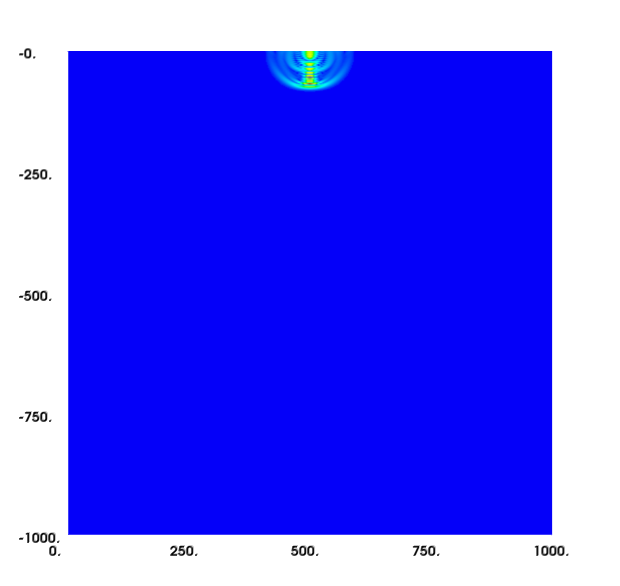
\includegraphics[width=3in]{figures/ex08pw50.png}
\label{fig:ex08pw50}
}
\subfigure[Example 08a at 0.175s ]{
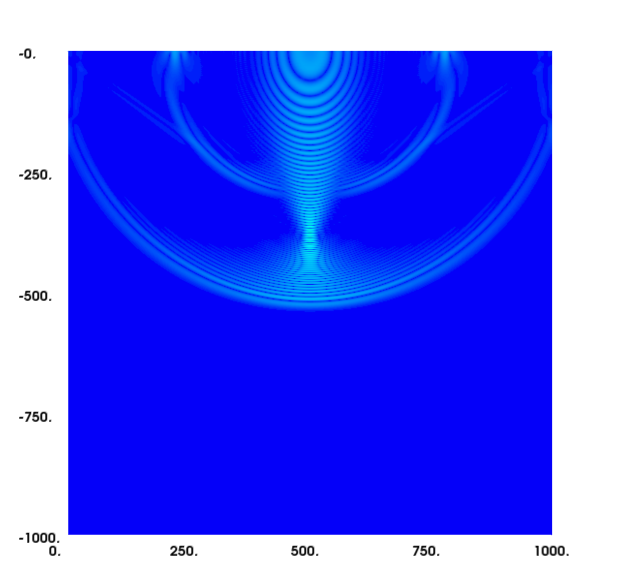
\includegraphics[width=3in]{figures/ex08pw350.png}
\label{fig:ex08pw350}
} \\
\subfigure[Example 08a at 0.325s ]{
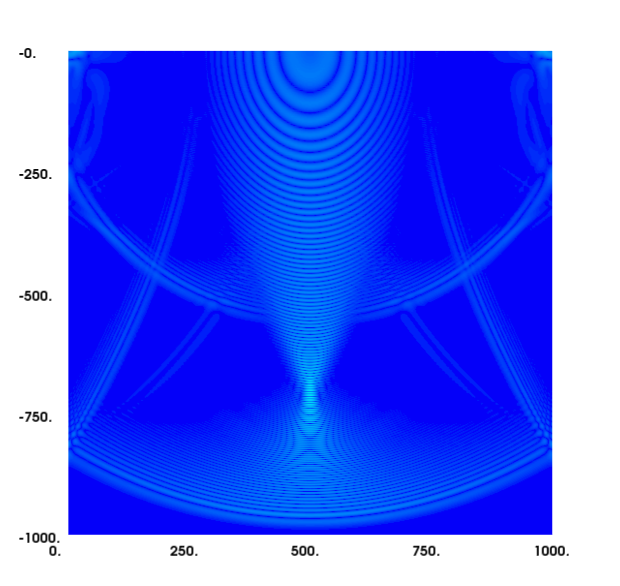
\includegraphics[width=3in]{figures/ex08pw650.png}
\label{fig:ex08pw650}
}
\subfigure[Example 08a at 0.475s ]{
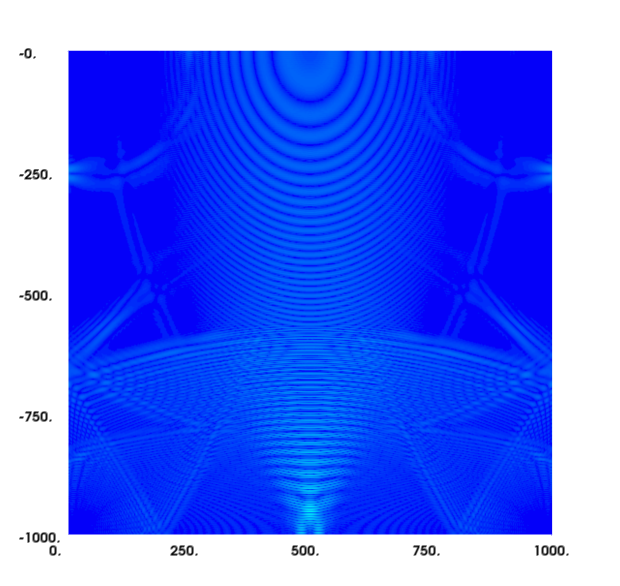
\includegraphics[width=3in]{figures/ex08pw950.png}
\label{fig:ex08pw950}
}
\label{fig:ex08pw}
\caption{Results of Example 08 at various times.}
\end{figure}
\clearpage

\section{Time variant source}

\sslist{example08b.py}
Until this point, all of the wave propagation examples in this cookbook have
used impulsive sources which are smooth in space but not time. It is however,
advantageous to have a time smoothed source as it can reduce the temporal
frequency range and thus mitigate aliasing in the solution. 

It is quite 
simple to implement a source which is smooth in time. In addition to the
original source function the only extra requirement is a time function. For
this example the time variant source will be the derivative of a gausian curve
defined by the required dominant frequency (\refig{fig:tvsource}).
\begin{python}
#Creating the time function of the source.
dfeq=50 #Dominant Frequency
a = 2.0 * (np.pi * dfeq)**2.0
t0 = 5.0 / (2.0 * np.pi * dfeq)
srclength = 5. * t0
ls = int(srclength/h)
print 'source length',ls
source=np.zeros(ls,'float') # source array
ampmax=0
for it in range(0,ls):
    t = it*h
    tt = t-t0
    dum1 = np.exp(-a * tt * tt)
    source[it] = -2. * a * tt * dum1
    if (abs(source[it]) > ampmax):
        ampmax = abs(source[it])
    time[t]=t*h
\end{python}
\begin{figure}[ht]
\centering
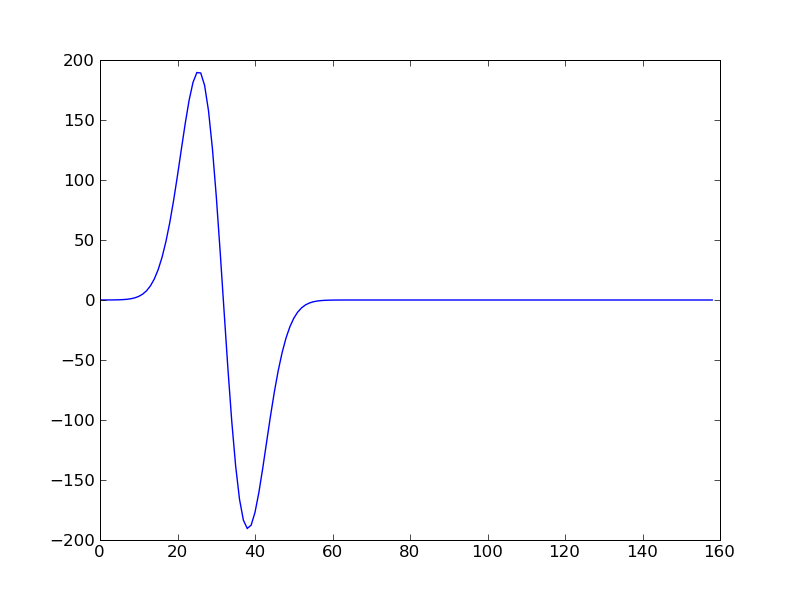
\includegraphics[width=3in]{figures/source.png}
\caption{Time variant source with a dominant frequency of 50Hz.}
\label{fig:tvsource}
\end{figure}

We then build the source and the first two time steps via;
\begin{python}
# set initial values for first two time steps with source terms
y=source[0]
*(cos(length(x-xc)*3.1415/src_length)+1)*whereNegative(length(x-xc)-src_length)
src_dir=numpy.array([0.,-1.]) # defines direction of point source as down
y=y*src_dir
mypde.setValue(y=y) #set the source as a function on the boundary
# initial value of displacement at point source is constant (U0=0.01)
# for first two time steps
u=[0.0,0.0]*whereNegative(x)
u_m1=u
\end{python}

Finally, for the length of the source, we are required to update each new
solution in the itterative section of the solver. This is done via;
\begin{python}
# increment loop values
t=t+h; n=n+1
if (n < ls):
	y=source[n]**(cos(length(x-xc)*3.1415/src_length)+1)*\
                   whereNegative(length(x-xc)-src_length)
        y=y*src_dir; mypde.setValue(y=y) #set the source as a function on the
boundary
\end{python}

\section{Absorbing Boundary Conditions}
To mitigate the effect of the boundary on the model, absorbing boundary
conditions can be introduced. These conditions effectively dampen the wave
energy as they approach the bounday and thus prevent that energy from being
reflected. This type of approach is used typically when a model only represents
a small portion of the entire model, which in reality may have infinite bounds.
It is inpractical to calculate the solution for an infinite model and thus ABCs
allow us the create an approximate solution with small to zero boundary effects
on a model with a solvable size. 

To dampen the waves, the method of Cerjan(1985)
\footnote{\textit{A nonreflecting boundary condition for discrete acoustic and
elastic wave equations}, 1985, Cerjan C, Geophysics 50, doi:10.1190/1.1441945}
where the solution and the stress are multiplied by a damping function defined
on $n$ nodes of the domain adjacent to the boundary, given by;
\begin{equation}
\gamma =\sqrt\left(\frac{|-log(\gamma\hackscore{b})|}{n^2}\right)
\end{equation}
\begin{equation}
y=e^{-(\gamma x)^2}
\end{equation}
This is applied to the bounding 20-50 pts of the model using the location
specifiers of \esc;
\begin{python}
# Define where the boundary decay will be applied.
bn=30.
bleft=xstep*bn; bright=mx-(xstep*bn); bbot=my-(ystep*bn)
# btop=ystep*bn # don't apply to force boundary!!!

# locate these points in the domain
left=x[0]-bleft; right=x[0]-bright; bottom=x[1]-bbot

tgamma=0.98   # decay value for exponential function
def calc_gamma(G,npts):
    func=np.sqrt(abs(-1.*np.log(G)/(npts**2.)))
    return func

gleft  = calc_gamma(tgamma,bleft)
gright = calc_gamma(tgamma,bleft)
gbottom= calc_gamma(tgamma,ystep*bn)

print 'gamma', gleft,gright,gbottom

# calculate decay functions
def abc_bfunc(gamma,loc,x,G):
    func=exp(-1.*(gamma*abs(loc-x))**2.)
    return func

fleft=abc_bfunc(gleft,bleft,x[0],tgamma)
fright=abc_bfunc(gright,bright,x[0],tgamma)
fbottom=abc_bfunc(gbottom,bbot,x[1],tgamma)
# apply these functions only where relevant
abcleft=fleft*whereNegative(left)
abcright=fright*wherePositive(right)
abcbottom=fbottom*wherePositive(bottom)
# make sure the inside of the abc is value 1
abcleft=abcleft+whereZero(abcleft)
abcright=abcright+whereZero(abcright)
abcbottom=abcbottom+whereZero(abcbottom)
# multiply the conditions together to get a smooth result
abc=abcleft*abcright*abcbottom
\end{python}
Note that the boundary conditions are not applied to the surface, as this is
effectively a free surface where normal reflections would be experienced.
Special conditions can be introduced at this surface if they are known. The
resulting boundary damping function can be viewed in Figure
\ref{fig:abconds}.

\section{Second order Meshing}
For stiff problems like the wave equation it is often prudent to implement
second order meshing. This creates a more accurate mesh approximation with some
increased processing cost. To turn second order meshing on, the \verb!rectangle!
function accpets an \verb!order! keyword argument.
\begin{python}
domain=Rectangle(l0=mx,l1=my,n0=ndx, n1=ndy,order=2) # create the domain
\end{python}
Other pycad functions and objects have similar keyword arguments for higher
order meshing.

Note that when implementing second order meshing, a smaller timestep is required
then for first order meshes as the second order essentially reduces the size of
the mesh by half.

\begin{figure}[ht]
 \centering
 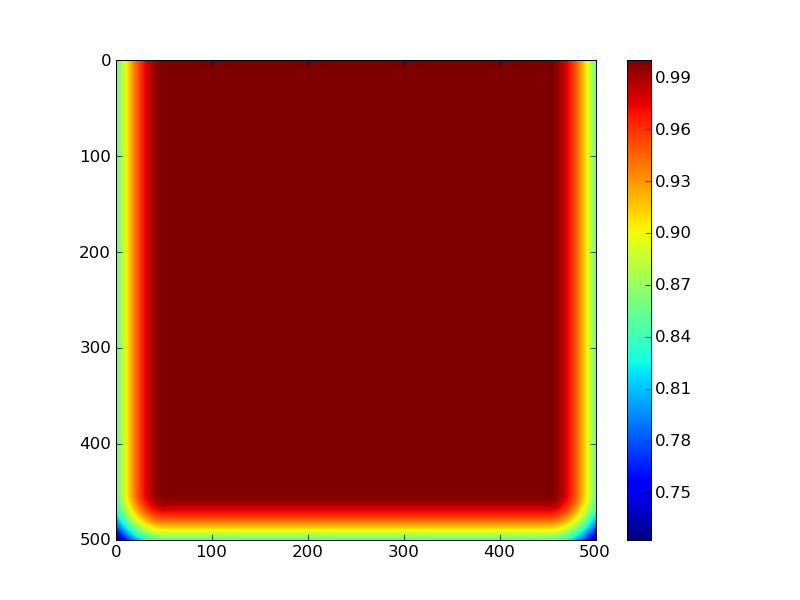
\includegraphics[width=5in]{figures/ex08babc.png}
 \label{fig:abconds}
 \caption{Absorbing boundary conditions for example08b.py}
\end{figure}

\begin{figure}[htp]
\centering
\subfigure[Example 08b at 0.03s ]{
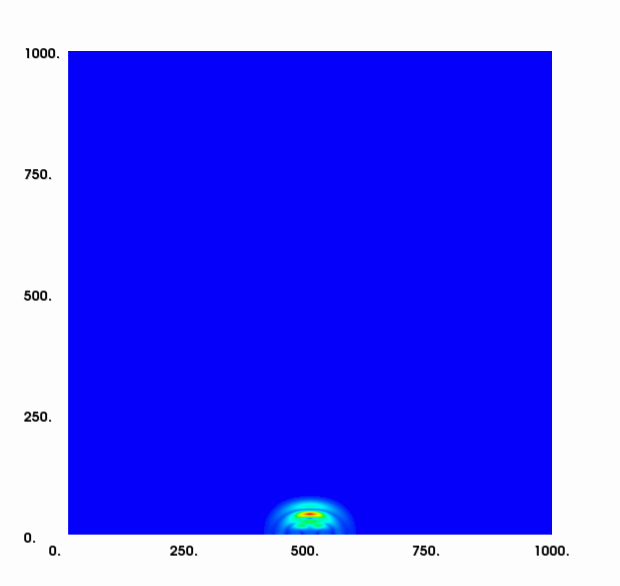
\includegraphics[width=3in]{figures/ex08sw060.png}
\label{fig:ex08pw060}
}
\subfigure[Example 08b at 0.16s ]{
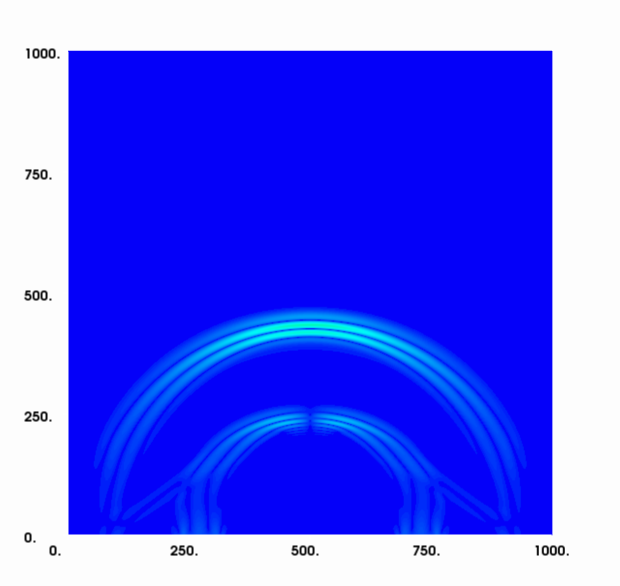
\includegraphics[width=3in]{figures/ex08sw320.png}
\label{fig:ex08pw320}
} \\
\subfigure[Example 08b at 0.33s ]{
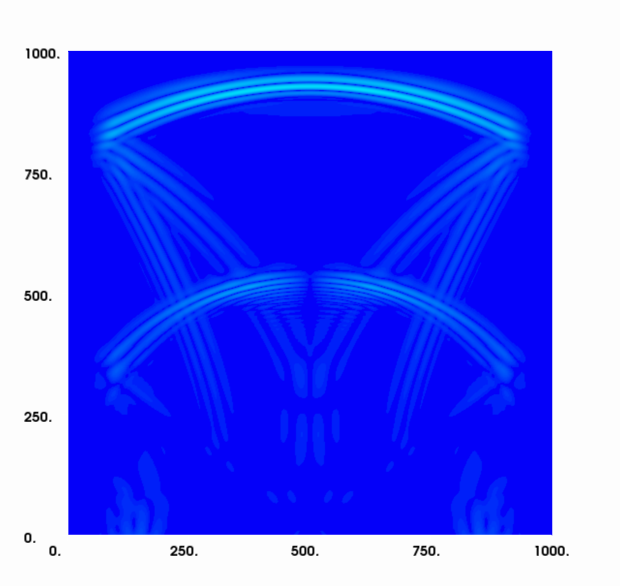
\includegraphics[width=3in]{figures/ex08sw660.png}
\label{fig:ex08pw660}
}
\subfigure[Example 08b at 0.44s ]{
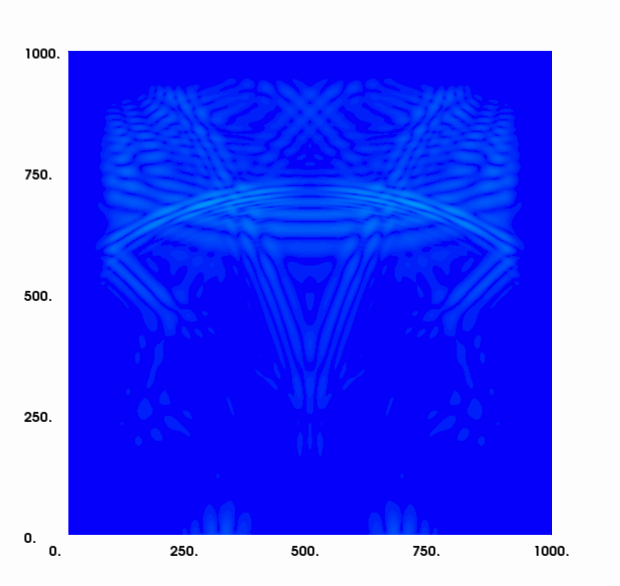
\includegraphics[width=3in]{figures/ex08sw880.png}
\label{fig:ex08pw880}
}
\label{fig:ex08pw}
\caption{Results of Example 08b at various times.}
\end{figure}
\clearpage

\section{Pycad example}
\sslist{example08c.py}
To make the problem more interesting we will now introduce an interface to the
middle of the domain. Infact we will use the same domain as we did for heat flux
in Chapter \ref{CHAP HEAT 2}. The domain contains a syncline with two set of
material properties on either side of the interface.

\begin{figure}[ht]
\begin{center}
%\includegraphics[width=5in]{figures/example08cgeo.png}
%Fix this.
\caption{Domain geometry for example08c.py showing line tangents.}
\label{fig:ex08cgeo}
\end{center}
\end{figure}

It is simple enough to slightly modify the scripts of the previous sections to
accept this domain. Multiple material parameters must now be deined and assigned
to specific tagged areas. Again this is done via
\begin{python}
lam=Scalar(0,Function(domain))
lam.setTaggedValue("top",lam1)
lam.setTaggedValue("bottom",lam2)
mu=Scalar(0,Function(domain))
mu.setTaggedValue("top",mu1)
mu.setTaggedValue("bottom",mu2)
rho=Scalar(0,Function(domain))
rho.setTaggedValue("top",rho1)
rho.setTaggedValue("bottom",rho2)
\end{python}
Don't forget that teh source boudnary must also be tagged and added so it can be
referenced 
\begin{python}
# Add the subdomains and flux boundaries.
d.addItems(PropertySet("top",tblock),PropertySet("bottom",bblock),\
                                     PropertySet("linetop",l30))
\end{python}
It is now possible to solve the script as in the previous examples.

\begin{figure}[ht]
\centering
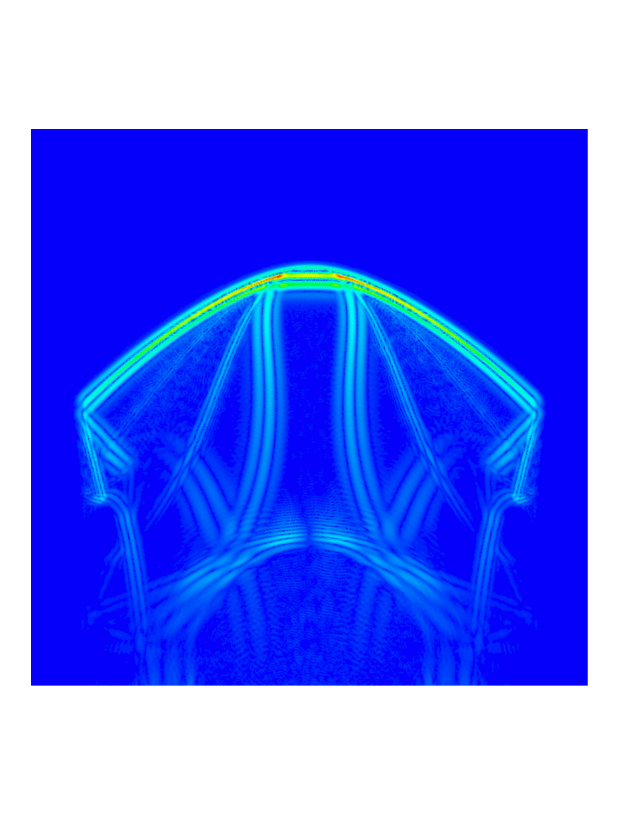
\includegraphics[width=4in]{figures/ex08c2601.png}
\caption{Modelling results of example08c.py at 0.2601 seconds. Notice the
refraction of the wave front about the boundary between the two layers.}
\label{fig:ex08cres}
\end{figure}


